
\documentclass[10pt]{article}

\usepackage{graphicx,amsmath,amssymb,subfigure,enumerate,versions}
\usepackage{multicol,multirow,mdframed}
\usepackage{epstopdf}
\usepackage{pstricks,auto-pst-pdf}
\usepackage{pst-all}
\usepackage{pst-ode}
\usepackage{pst-math}
\usepackage{hyperref}
\usepackage{listings}
%\usepackage{mcode}
\lstset{language=Matlab}
\DeclareGraphicsExtensions{.png,.jpg,.pdf}

% ************ Page Margins *************
\hoffset=-1.3in
\setlength{\textwidth}{7.5in}
%%%%% MARGINS
\topmargin 0pt
\advance \topmargin by -\headheight
\advance \topmargin by -\headsep
\textheight 9.5in

% ************ Shortcuts *************
\newcommand{\Z}{\mbox{\sf Z\hspace{-1.5mm}Z}}
\newcommand{\SolutionSeparator}{ \hfill \hfill \hrule \hfill \hfill }
\newcommand{\R}{\mbox{\rm I\hspace{-0.75mm}R}}
\columnsep=0.75in
\newcommand{\vsc}{\vspace{1mm}}
\newcommand{\D}{\Delta }
\newcommand{\ifd}{f(x)~dx}
\newcommand{\dd}{\frac{dy}{dx} \,} 
\newcommand{\der}[2]{\frac{d{#1}}{d{#2}} \,}
\newcommand{\ddx}[1]{\frac{d {#1}}{dx} \,} 
\newcommand{\ddy}[1]{\frac{d {#1}}{dy} \,} 
\newcommand{\ddz}[1]{\frac{d {#1}}{dz} \,} 
\newcommand{\ddt}[1]{\frac{d {#1}}{dt} \,} 
\newcommand{\ds}{\displaystyle } 
\newcommand{\la}{\lambda } 
\newcommand{\del}{\nabla } 
\newcommand{\zx}{\frac{\partial z}{\partial x} \,}
\newcommand{\zy}{\frac{\partial z}{\partial y} \,}
\newcommand{\dx}{\frac{\partial f}{\partial x} \,}
\newcommand{\dy}{\frac{\partial f}{\partial y} \,}
\newcommand{\pp}[2]{\frac{\partial {#1}}{\partial {#2}} \,}
\newcommand{\ppx}{\frac{\partial }{\partial x} \,}
\newcommand{\ppy}{\frac{\partial }{\partial y} \,}
\renewcommand{\thesection}{\Roman{section}}
\newcommand{\vi}{\vec{i}}
\newcommand{\vj}{\vec{j}}
\newcommand{\vk}{\vec{k}}
\newcommand{\vv}{\vec{v}}
\newcommand{\lan}{\left\langle}
\newcommand{\ran}{\right\rangle}
\newcommand{\degr}{^{\circ}}

% *** Define the printed question style ***
\newcommand{\q}[1]{ {\em #1} }
% \renewcommand{\q}[1]{ {} }

\newcommand{\notice}{ \begin{center}Some problems and solutions
    selected or adapted from \\ Stewart {\em Calculus-Early
      Transcendentals} and Hughes-Hallett {\em Calculus} .\end{center}
}

% *** Overwrite, if desired, the question format
\includeversion{Question} 
\includeversion{Solution}

\newcommand{\multicolstart}{ }
\newcommand{\multicolend}{ }

\renewenvironment{Question}
{ \begin{mdframed}[nobreak=true,hidealllines=true,backgroundcolor=gray!50,innerleftmargin=5ex] }
{ \end{mdframed} }


% *** Footnoting with symbols ***
\long\def\symbolfootnote[#1]#2{\begingroup%
\def\thefootnote{\fnsymbol{footnote}}\footnote[#1]{#2}\endgroup}

\newcommand{\WeekTitleOne}{Derivatives - Foundations}
\newcommand{\WeekTitleTwo}{Derivatives - Linearization and Applications}
\newcommand{\WeekTitleThree}{Derivatives - Modeling}
\newcommand{\WeekTitleFour}{Integrals - Foundations}
\newcommand{\WeekTitleFive}{Integrals - Techniques}
\newcommand{\WeekTitleSix}{Integrals - Modeling}
\newcommand{\WeekTitleSeven}{Differential Equations - }
\newcommand{\WeekTitleEight}{Differential Equations - }
\newcommand{\WeekTitleNine}{Differential Equations - }
\newcommand{\WeekTitleTen}{Linear Algebra - }
\newcommand{\WeekTitleEleven}{Linear Algebra - }
\newcommand{\WeekTitleTwelve}{Linear Algebra - }


\begin{document}

\begin{center}
\subsection*{MNTC P01 - Week \#7 - \WeekTitleSeven}
\end{center}

\begin{enumerate}

\subsection*{Verifying Solutions}
% ******************************
\item 
\begin{Question} %9.1 - 1
  Show that $\ds y = \frac{2}{3}\text{e}^{x} + \text{e}^{-2x}$ is a solution of the differential equation $y' + 2y = 2\text{e}^{x}$. \\
\end{Question}

% 1 - Solution
\begin{Solution}
\begin{equation*}
y = \frac{2}{3}\text{e}^{x} + \text{e}^{-2x} \Rightarrow
y' = \frac{2}{3}\text{e}^{x} - 2\text{e}^{-2x}
\end{equation*}
To show that $y$ is a solution of the differential equation, we will substitute the expressions for $y$ and $y'$ in the left-hand side of the equation and show that the left-hand side of the equation and show that the left-hand side is equal to the right-hand side.

\begin{align*}
	\text{LHS} &= y' + 2y = \frac{2}{3}\text{e}^{x} - 2\text{e}^{-2x} + 2(\frac{2}{3}\text{e}^{x} + \text{e}^{-2x}) \\
	&= \frac{2}{3}\text{e}^{x} - 2\text{e}^{-2x} + 
	\frac{4}{3}\text{e}^{x} + 2\text{e}^{-2x} =
	\frac{6}{3}\text{e}^{x} = 2\text{e}^{x} \\ 
	&= \text{RHS}
\end{align*}
\end{Solution}
%%%%%%%%%%%%%%%%%%

%9.1 - 3
\item
\begin{Question}
\begin{enumerate}[(a)]
\item For what values of $r$ does the function $y = \text{e}^{rx}$ satisfy the differential equation $2y'' + y' - y = 0$?

\item If $r_1$ and $r_2$ are the values of $r$ that you found in part (a), show that every member of the family of functions $y = a\text{e}^{r_{1}x} + b\text{e}^{r_{2}x}$ is also a solution.
\end{enumerate}
\end{Question}

\begin{Solution}
\begin{enumerate}[(a)]
\item \begin{equation*}
		y = \text{e}^{rx} \Rightarrow
		y' = r\text{e}^{rx} \Rightarrow
		y'' = r^2\text{e}^{rx}
	\end{equation*}
	Substituting these expressions into the differential equation 
	$2y'' + y' - y = 0$, we get
	\begin{align*}
		&2r^2\text{e}^{rx} + r\text{e}^{rx} - \text{e}^{rx} = 0 \\
		\Rightarrow \quad &(2r^2 + r - 1)\text{e}^{rx} = 0 \\
		\Rightarrow \quad &(2r - 1)(r + 1) = 0
	\end{align*}
	(since $\text{e}^{rx}$ is never zero) $r = \frac{1}{2}$ or -1.

\item Let $r_1 = \frac{1}{2}$ and $r_2 = -1$, so we need to show that every member of the family of functions $y = a\text{e}^{x/2} + b\text{e}^{-x}$ is a solution of the differential equation $2y'' + y' - y = 0$.\\
\begin{align*}
	&y = a\text{e}^{x/2} + b\text{e}^{-x} \\
	\Rightarrow \quad &y' = \frac{1}{2}a\text{e}^{x/2} - b\text{e}^{-x}\\
	\Rightarrow \quad &y'' = \frac{1}{4}a\text{e}^{x/2} + b\text{e}^{-x}
\end{align*}
\begin{align*}
	\text{LHS} &= 2y'' + y' - y \\ 
	&= 2(\frac{1}{4}a\text{e}^{x/2} + b\text{e}^{-x}) + (\frac{1}{2}a\text{e}^{x/2} - b\text{e}^{-x}) \\ & \hspace{4mm}- (a\text{e}^{x/2} + b\text{e}^{-x}) \\
	&= \frac{1}{2}a\text{e}^{x/2} + 2b\text{e}^{-x} + \frac{1}{2}a\text{e}^{x/2} - b\text{e}^{-x}  \\
	& \hspace{4mm}- a\text{e}^{x/2} - b\text{e}^{-x} \\
	&= (\frac{1}{2}a + \frac{1}{2}a - a)\text{e}^{x/2} + (2b - b -b)\text{e}^{-x} \\
	&= 0 \\ &= \text{RHS}
\end{align*}
\end{enumerate}
\end{Solution}
%%%%%%%%%%%%%%%%%%

%9.1 - 4
\item
\begin{Question}
\begin{enumerate}[(a)]
\item For what values of $k$ does the function $y = \cos(kt)$ satisfy
  the differential equation $4y'' = -25y$?
\item For those values of $k$, verify that every member of the vamily of functions $y = A\sin kt + B\cos kt$ is also a solution.
\end{enumerate}
\end{Question}

\begin{Solution}
\begin{enumerate}[(a)]
\item \begin{equation*}
		y = \cos kt \ \Rightarrow \ y' = -k \sin kt \ \Rightarrow \ y'' = -k^2 \cos kt
	\end{equation*}
	Substituting expressions into the differential equation $4y'' = -25y$, we get 
	\begin{align*}
		&4(-k^2\cos kt) = -25(\cos kt) \\
		\Rightarrow \quad &(25 - 4k^2) \cos kt = 0 (\text{for all } t)\\
		\Rightarrow \quad &25 - 4k^2 = 0 \\
		\Rightarrow \quad &k^2 = \frac{25}{4} \ \Rightarrow \ k = \pm \frac{5}{2}
	\end{align*}
	
\item \begin{align*}
		&y = A\sin kt + B \cos kt \\
		\Rightarrow \quad &y' = Ak\cos kt - Bk \sin kt \\
		\Rightarrow \quad &y'' = -Ak^2 \sin kt - Bk^2 \cos kt
	\end{align*}
	The given differential equation $4y'' = -25y$ is equivalent to $4y'' + 25y = 0$.  Thus,
\begin{align*}
	\text{LHS} &= 4y'' + 25y \\
	&= 4(-Ak^2 \sin kt - Bk^2 \cos kt) \\
	& \quad + 25(A\sin kt + B\cos kt) \\
	&= -4Ak^2 \sin kt - 4Bk^2 \cos kt \\
	& \quad+ 25A\sin kt + 25B \cos kt \\
	&= (25 - 4k^2)A\sin kt + (25 - 4k^2)B\cos kt \\
	&= 0 \hspace{4mm} \text{since } k^2 = \frac{25}{4}
\end{align*}
\end{enumerate}
\end{Solution}
%%%%%%%%%%%%%%%%%%

%9.1 - 7
\item
\begin{Question}
  Consider the differential equation $\ds \frac{dy}{dx} = -y^2$.
\begin{enumerate}[(a)]
\item If you were asked whether the solutions to this equation would
  {\em increase} or {\em decrease} as $x$ increased, what could you
  say based on only the equation itself?
\item Verify that all members of the family $y = 1/(x + C)$ are
  solutions of the equation in part (a).
\item Can you think of a (very simple) solution of the differential
  equation $y' = -y^2$ that is {\em not} a member of the family in
  part (b)?
\item Find the solution to the initial-value problem
\begin{equation*}
	y' = -y^2 \hspace{6mm} y(0) = 0.5
\end{equation*}
\end{enumerate}
\end{Question}
\begin{Solution}
\begin{enumerate}[(a)]
\item Since the derivative of $y' = -y^2$ is always negative (or 0 if
  $y = 0$), the function $y$ must be {\bf decreasing} (or maybe
  horizontal) on any interval on which it is defined.
\item We sub in the proposed solution into the original equation.  To do this, we will need the derivative of $y$:  $\ds y = \frac{1}{x + C} \Rightarrow y' = -\frac{1}{(x + C)^2}$.\\
  $\text{LHS} = y' = -\frac{1}{(x + C)^2} = -\left(\frac{1}{x + C}
  \right)^2 = -y^2 = \text{RHS}$ Therefore, any function of the form
  $y(x) = \frac{1}{x+C}$ {\bf is} a solution to $y' = -y^2$.
\item $y=0$ is a simple solution to $y'=-y^2$ that is not a member of
  the family in part (b).  We can confirm this by subbing $y=0$ into
  the DE and checking the LHS equals the RHS.  If $y=0$, then $y'= 0$
  as well, so $\text{LHS} = y' = 0 = -y^2 = RHS$.
\item We already know that the solutions will be of the form
  $y(x) = \frac{1}{x+C}$; we just need to sub in the initial value to
  solve for $C$.

  If $y(x) = \frac{1}{x + C}$, then
  $y(0) = \frac{1}{0 + C} = \frac{1}{C}$.  Since $y(0) = 0.5$,
  $\frac{1}{C} \frac{1}{2} \Rightarrow C = 2$, so $y =\frac{1}{x + 2}$
\end{enumerate}
\end{Solution}
%%%%%%%%%%%%%%%%%%

\hrulefill

\subsection*{Numerical ODE Solutions With MATLAB}


%*******************************
\item
\begin{Question}
  Create a plot for the solution to the differential equation
  $y' - \frac{y^2}{x^3} = 0$ if y(2) = 1.  Include a large enough
  \verb#xspan# to see the long-term behaviour.
\end{Question}

\begin{Solution}
  For this first example of use MATLAB to build a numerical solution
  to a DE, we will show the full listing of a script that generates a
  solution to the given differential equation.  In later solutions, we
  will only include the key lines for the MATLAB script.

  Notes: 
  \begin{itemize}
  \item We set \verb#xspan# to start at 2 in the line
    \verb#xspan = [2, 30]#.  This is used because the solution MATLAB
    is generating will start at the coordinates $x_0$ = first element
    of \verb#xspan#, and $y_0$ = \verb#y0# in the code, and our
    initial condition is $x = 2$, $y=1$.
  \item We find the second value in the time span with some trial and
    error.  Any value larger than 15 or 20 would be sufficient to show
    the long-term trend in the solution.
  \end{itemize}
\lstinputlisting[showstringspaces=false]{MATLAB/W07DE01.m}

Link to the MATLAB code: \\
\href{http://www.mast.queensu.ca/~apsc171/MNTCP01/PracticeProblems/MATLAB/W07DE01.m}{W07DE01.m}

Here is the graph of the solution.

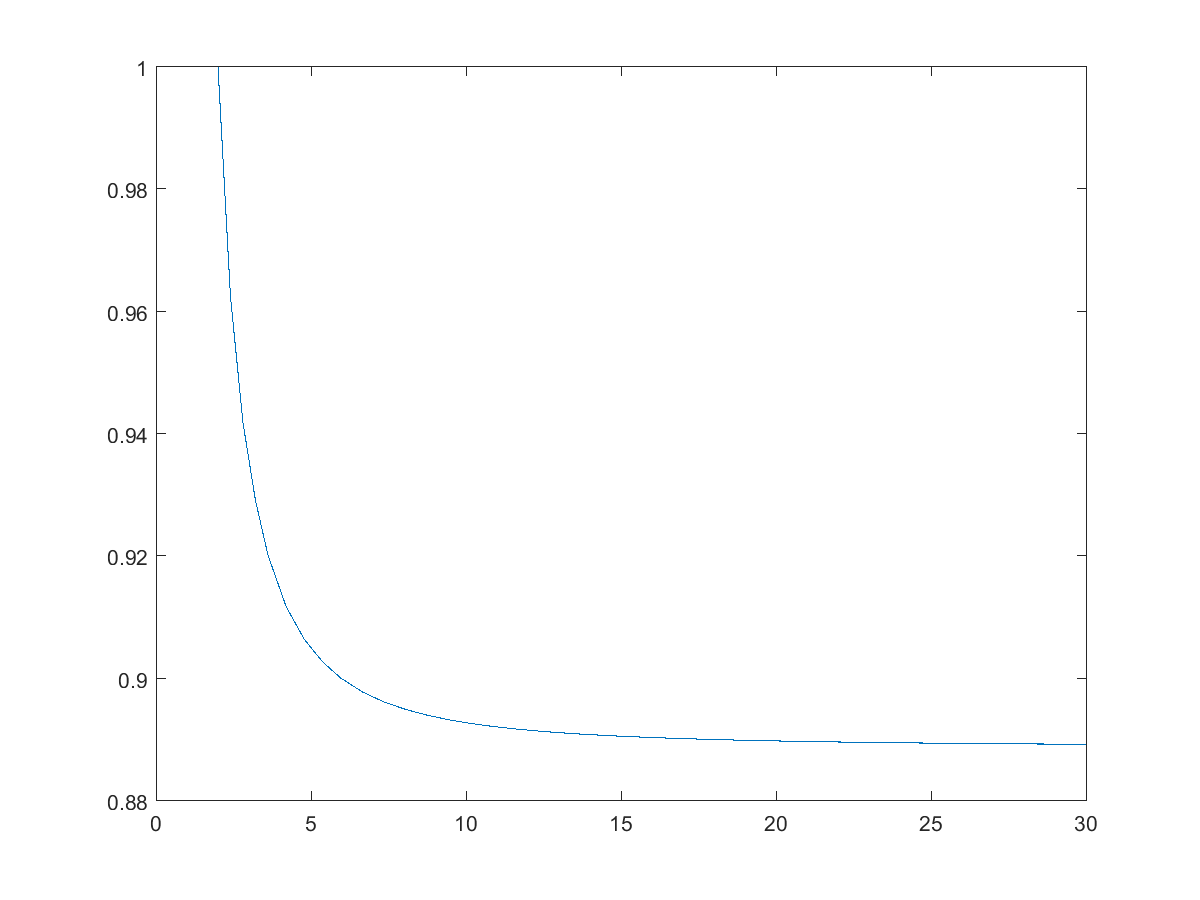
\includegraphics[width = 0.5\linewidth]{graphics/Week07_DESolutions/W07DE01}

    
\end{Solution}


%*******************************
\item
\begin{Question}
Create a plot for the solution to the differential equation
  $(2y - 4)y' - 3x^2 = 4x - 4$, if y(1) = 3.
    
\end{Question}

\begin{Solution}
  To generate a first-order DE solution in MATLAB, the differential
  equation must be written first in the form $y' = \ldots$.
  \begin{align*}
    (2y - 4)y' - 3x^2 & = 4x - 4 \\
    (2y - 4)y' & =  3x^2 +4x - 4 \\
    y' & =  \frac{(3x^2 +4x - 4)}{(2y - 4)} \\
  \end{align*}
    
Link to the MATLAB code: \\
\href{http://www.mast.queensu.ca/~apsc171/MNTCP01/PracticeProblems/MATLAB/W07DE02.m}{W07DE02.m}

Here is the graph of the solution.

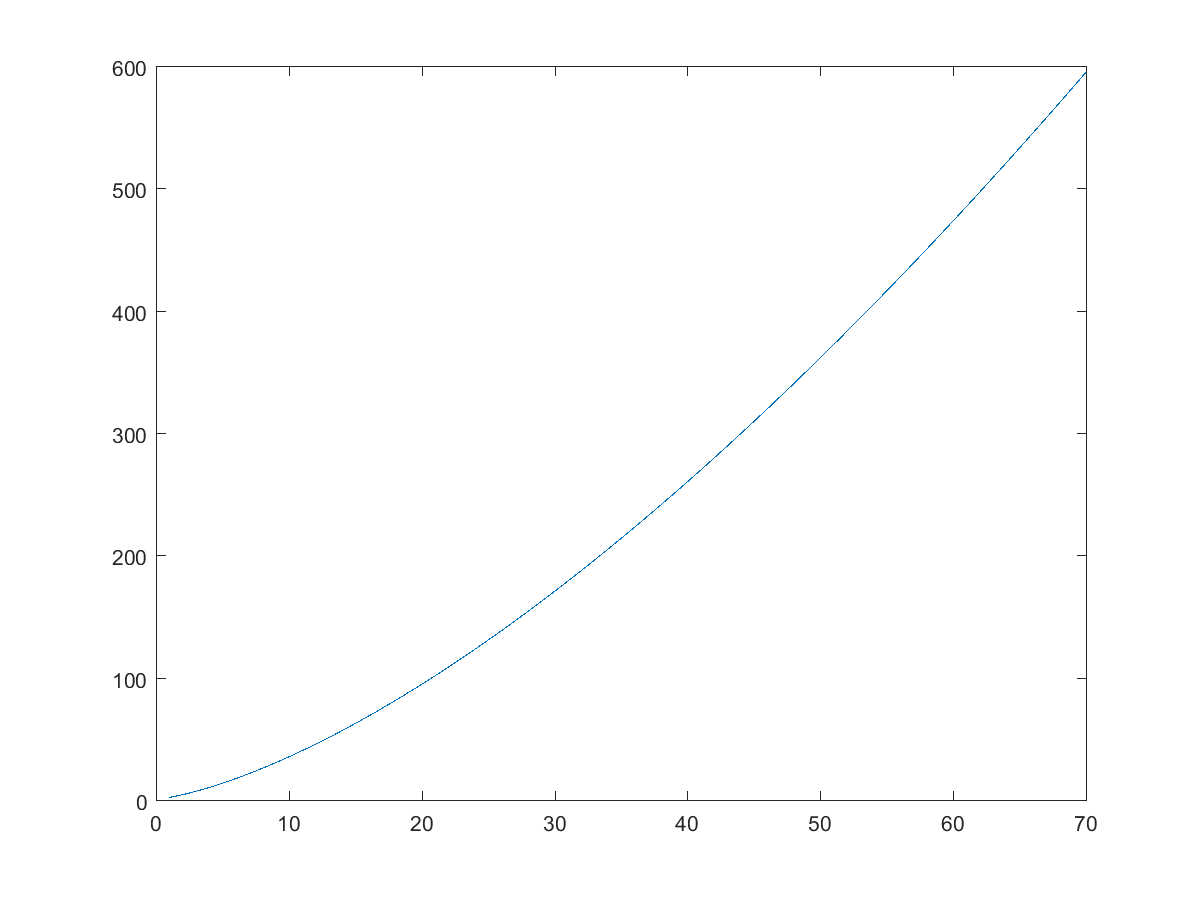
\includegraphics[width = 0.5\linewidth]{graphics/Week07_DESolutions/W07DE02}
\end{Solution}


%*******************************
\item
\begin{Question}
Create a plot for the solution to the differential equation
  $y' = e^{-y}(2t - 4)$ if $y(0) = 5$
    
\end{Question}

\begin{Solution}
  This DE is already in the form $y' = \ldots$, so we can input it
  into MATLAB as-is.  Note that the independent variable in this
  example is $t$, so we will use that in MATLAB instead of the
  variable $x$.


Link to the MATLAB code: \\
\href{http://www.mast.queensu.ca/~apsc171/MNTCP01/PracticeProblems/MATLAB/W07DE03.m}{W07DE03.m}

Here is the graph of the solution.

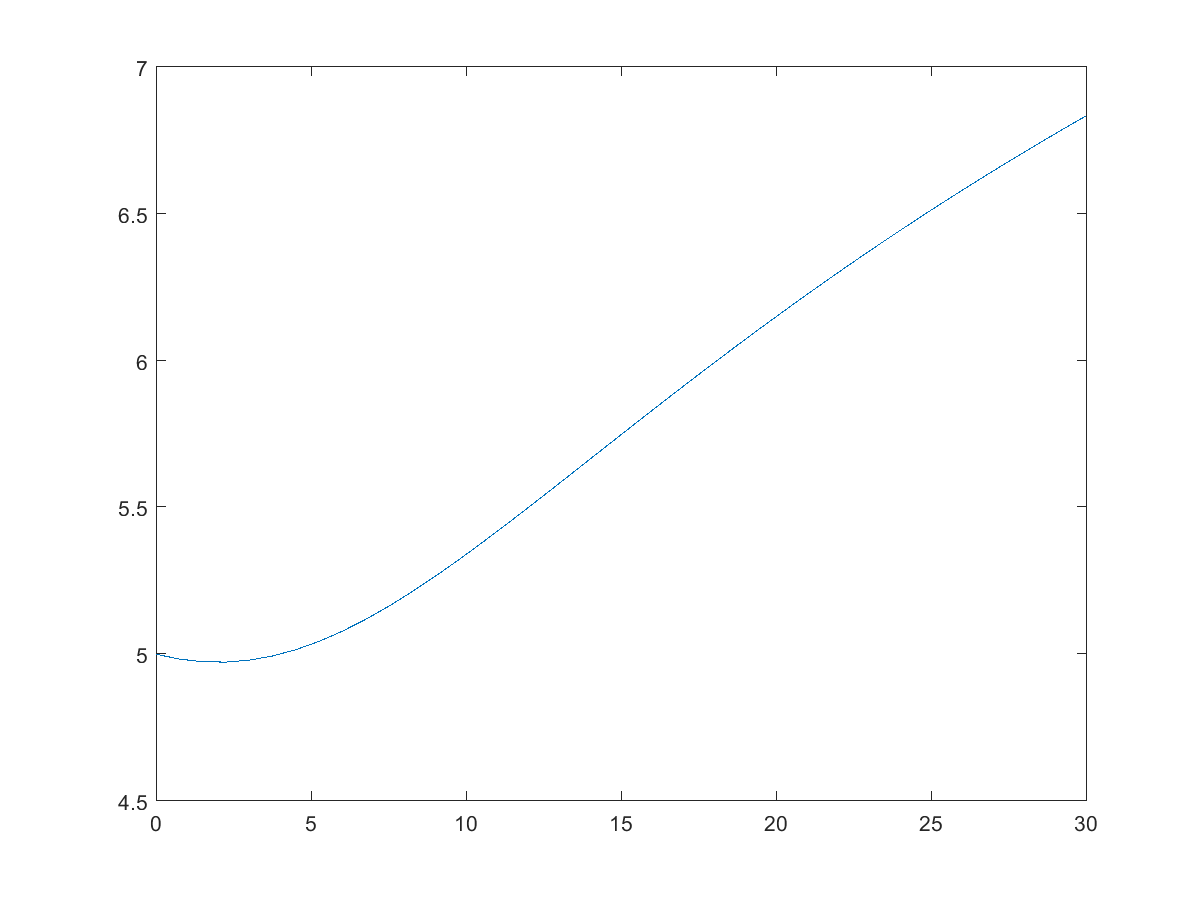
\includegraphics[width = 0.5\linewidth]{graphics/Week07_DESolutions/W07DE03}


    
\end{Solution}

%*******************************
\item
\begin{Question}
Create a plot for the solution to the differential equation
  $ty' - 2y = t^5 \sin (2t) - t^3 + 4t^4$, if
  $y(\pi) = \frac{3}{2}\pi^4$
    
\end{Question}

\begin{Solution}
  To generate a first-order DE solution in MATLAB, the differential
  equation must be written first in the form $y' = \ldots$.
  \begin{align*}
    ty' - 2y & = t^5 \sin (2t) - t^3 + 4t^4 \\
    ty' & = 2y + t^5 \sin(2t) - t^3 + 4t^4 \\
    y' & = \frac{1}{t} (2y + t^5 \sin(2t) - t^3 + 4t^4) \\
  \end{align*}
    
Link to the MATLAB code: \\
\href{http://www.mast.queensu.ca/~apsc171/MNTCP01/PracticeProblems/MATLAB/W07DE04.m}{W07DE04.m}

Here is the graph of the solution.

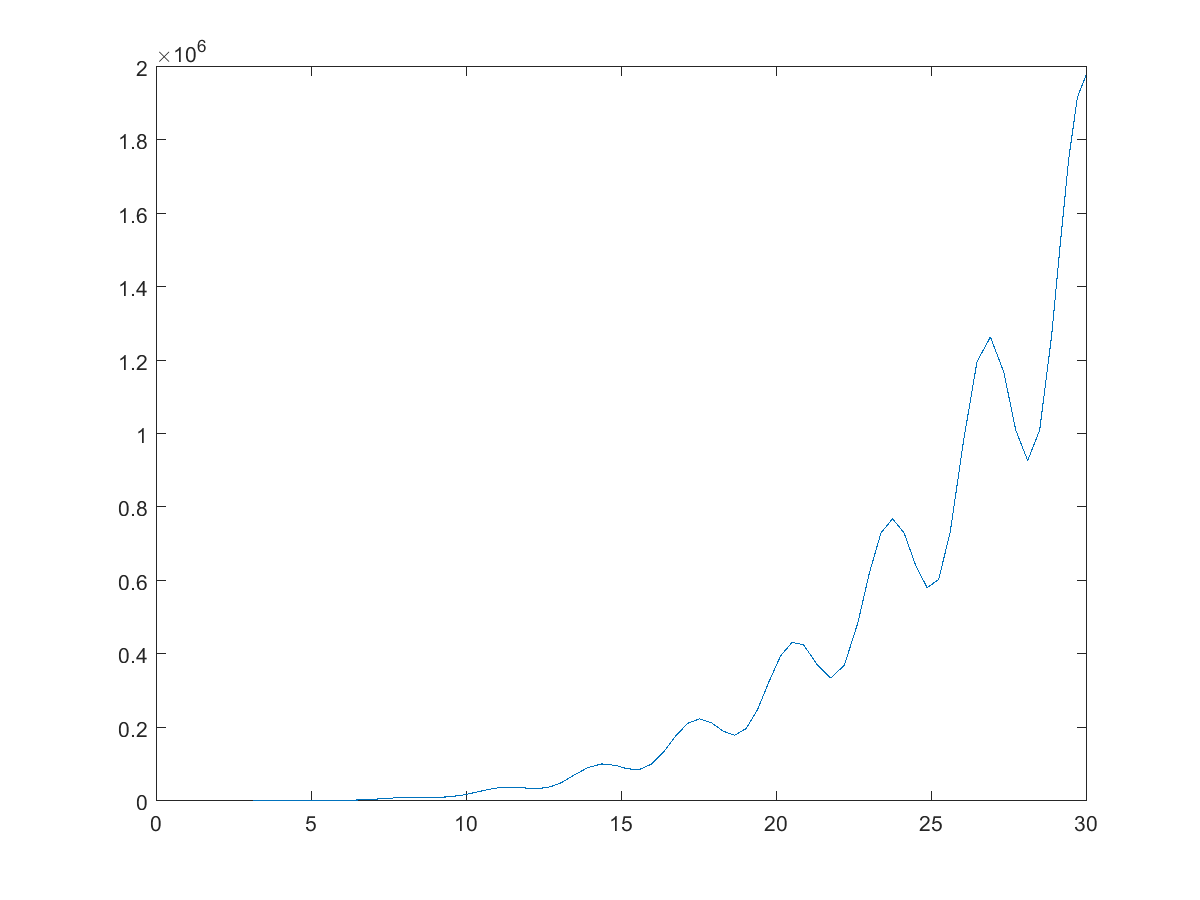
\includegraphics[width = 0.5\linewidth]{graphics/Week07_DESolutions/W07DE04}
    
Note that in this example, because of the $\sin(2t)$ introducing an
oscillation in the system, the solution won't look at simple as some
of the other examples.
\end{Solution}

%*******************************
\item
\begin{Question}
  Create a plot for the solution to the differential equation
  $ty' + 2y = t^2 - t + 1$, if $y(1) = 0.5$.
    
\end{Question}

\begin{Solution}
  To generate a first-order DE solution in MATLAB, the differential
  equation must be written first in the form $y' = \ldots$.
  \begin{align*}
    ty' + 2y = t^2 - t + 1 \\
    ty' = -2y + t^2 - t + 1 \\
    y' = \frac{1}{t} (-2y + t^2 - t + 1) \\
  \end{align*}
    
Link to the MATLAB code: \\
\href{http://www.mast.queensu.ca/~apsc171/MNTCP01/PracticeProblems/MATLAB/W07DE05.m}{W07DE05.m}

Here is the graph of the solution.

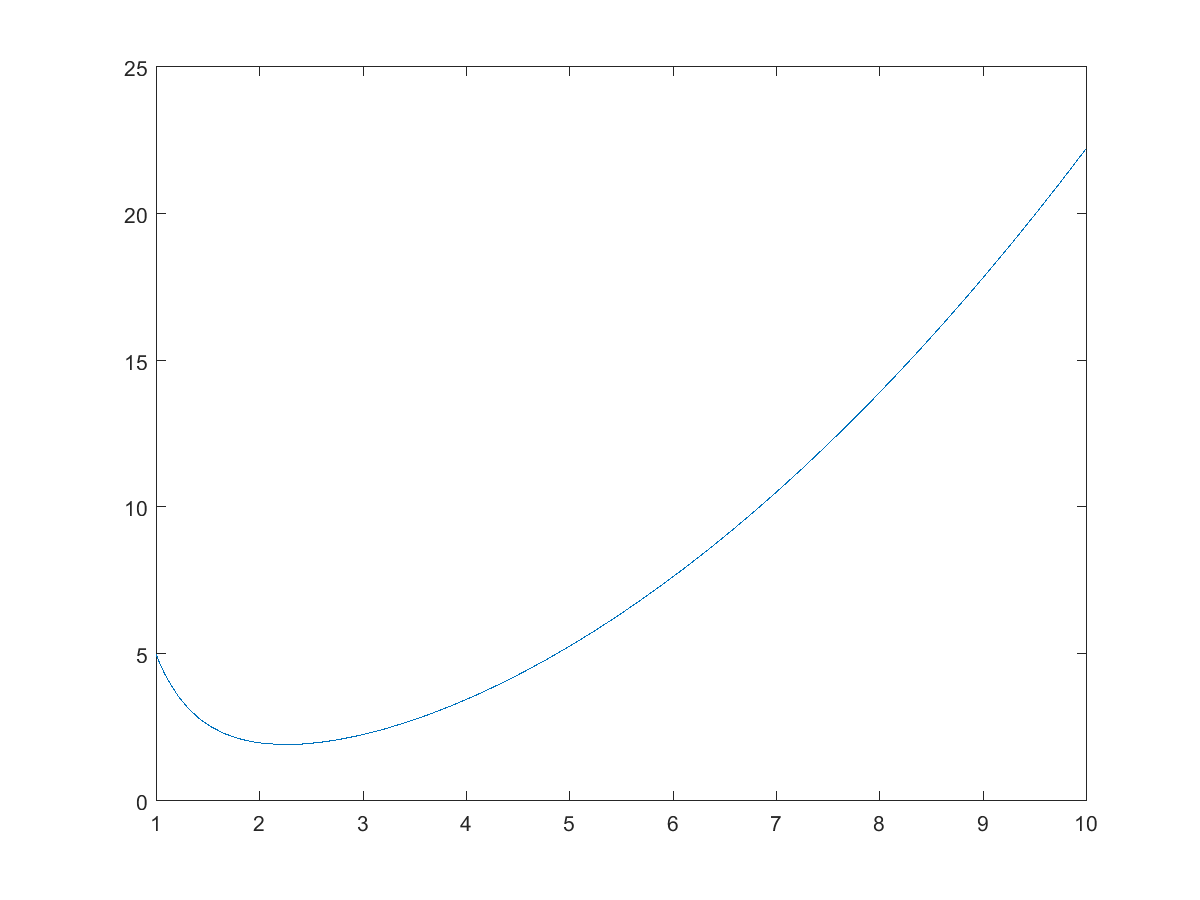
\includegraphics[width = 0.5\linewidth]{graphics/Week07_DESolutions/W07DE05}
    
    
\end{Solution}

%*******************************
\item
\begin{Question}
  Create a plot for the solution to the differential equation
  $2xy^2 + 4 = 2(3 - x^2y)y'$ if $y(5) = 8$.
    
\end{Question}

\begin{Solution}
  To generate a first-order DE solution in MATLAB, the differential
  equation must be written first in the form $y' = \ldots$.  We start
  by switching both sides of the equation to put $y'$ on the left.
  \begin{align*}
    2(3 - x^2y)y' & = 2xy^2 + 4   \\
    y' & = \frac{ 2xy^2 + 4}{2 (3-x^2 y)} 
  \end{align*}
    
Link to the MATLAB code: \\
\href{http://www.mast.queensu.ca/~apsc171/MNTCP01/PracticeProblems/MATLAB/W07DE06.m}{W07DE06.m}

Here is the graph of the solution.

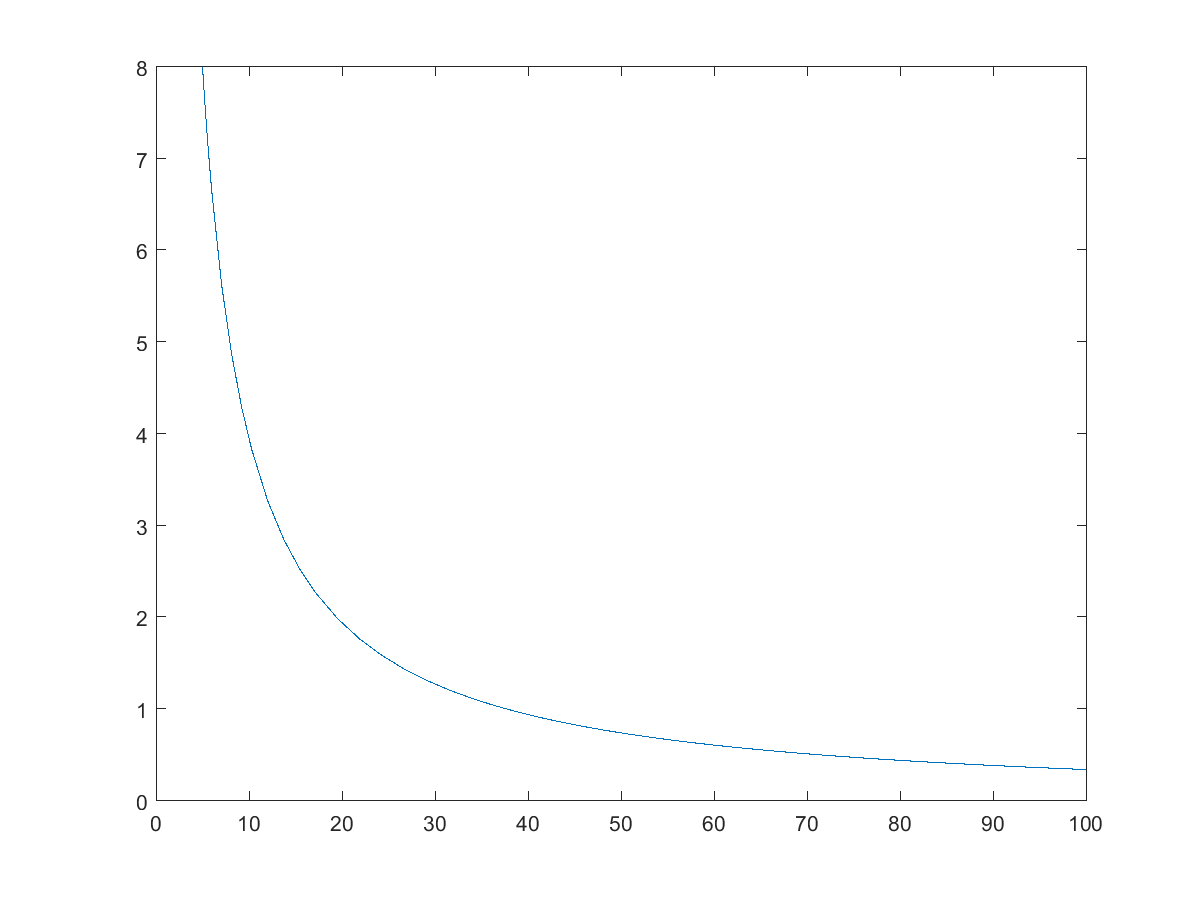
\includegraphics[width = 0.5\linewidth]{graphics/Week07_DESolutions/W07DE06}
    
    
\end{Solution}


\end{enumerate}





\end{document}
